\documentclass[bachelor, och, referat]{template}

\usepackage[utf8]{inputenc}
\usepackage{graphicx}

\usepackage{pdfpages}
\usepackage{amsmath}

\usepackage[sort,compress]{cite}
\usepackage{amsmath}
\usepackage{amssymb}
\usepackage{amsthm}
\usepackage{fancyvrb}
\usepackage{longtable}
\usepackage{array}
\usepackage[english,russian]{babel}
\usepackage{minted}

\usepackage{tempora}

\usepackage[justification=centering]{caption}
\usepackage[colorlinks=false, hidelinks=true]{hyperref}


\newcommand{\eqdef}{\stackrel {\rm def}{=}}


\begin{document}

\title{Нейронные иммунные сети}

\course{5}

\group{531}

\napravlenie{10.05.01 "--- Компьютерная безопасность}


\author{Токарева Никиты Сергеевича}


\satitle{доцент}
\saname{И.\,И.\, Слеповичев}


\date{2023}

\maketitle

% Включение нумерации рисунков, формул и таблиц по разделам
% (по умолчанию - нумерация сквозная)
% (допускается оба вида нумерации)
%\secNumbering


\tableofcontents

\intro
С развитием области компьютерных наук и техники общество столкнулось с 
возрастающей проблемой киберпреступности. Одним из аспектов этой проблемы 
является разработка и распространение вредоносных программ, известных как 
компьютерные вирусы. В настоящее время обеспечение защиты компьютерных 
систем от подобных вредоносных программ является приоритетным направлением 
в области обеспечения информационной безопасности. Традиционные методы, 
основанные на сигнатурном поиске для выявления компьютерных вирусов, 
эффективны в обнаружении известных угроз, но оказываются неэффективными 
при обнаружении неизвестных вредоносных программ. Время, проходящее с 
момента появления нового компьютерного вируса до его обнаружения 
специалистами антивирусной индустрии, может быть значительным, 
что позволяет современным вредоносным программам распространяться 
и причинять серьезные ущербы. Компьютерные системы с устаревшими 
антивирусными базами становятся беспомощными перед новыми угрозами. 
Эвристические анализаторы, используемые для обнаружения неизвестных 
компьютерных вирусов, на текущий момент далеки от идеальных и часто 
либо ложно классифицируют чистые, неинфицированные файлы как вредоносные 
программы, либо не распознают зловредные программы.

Данная работа представляет собой обзор нейронных иммунных сетей (НИС), в 
которых комбинируются искусственные иммунные системы (ИИС) и нейронные 
сети. В рамках исследования рассматривается взаимосвязь между биологической 
иммунной системой и искусственными иммунными системами, а также представлен 
механизм обнаружения вирусов с использованием ИИС.


\section{Искусственные иммунные системы} 
\subsection{Связь биологической иммунной системы с искусственными иммунными системами}

Механизмы, использующиеся в ис­кусственных иммунных системах, позволяют обнаруживать неизвестные
компьютерные вирусы. Искусственные иммунные системы (ИИС) 
базируются на основных принципах биологической иммунной системы (БИС) \cite{ais1}.

БИС является уникальной системой, которая ежедневно борется с болез­нетворными 
бактериями и вирусами, защищая организм от инфекций.
Уникальность БИС заключается в том, что она способна обнаруживать не
только известные вирусы и бактерии, но также и неизвестные. Иммунитет
основан на способности лимфоцитов распознавать собственные клетки
организма от чужеродных клеток.

Основными элементами иммунной системы являются лимфоциты – белые клетки.
Существуют две разновидности лимфоцитов, которые образуются из стволовых клеток в
костном мозге. После синтеза лимфоциты попадают в кровяное русло. Некоторые из них
направляются к тимусу (вилочковой железе), где происходит их созревание (Т-лимфоциты). 
Другие же попадают в лимфатические узлы, и их созревание происходит
там (В-лимфоциты). Процесс созревания незрелых лимфоцитов играет большую роль в
иммунной системе и называется селекцией антител. В результате селекции уничтожаются 
нежелательные для организма лимфоциты. Зрелые лимфоциты имеют на своей поверхности 
детекторы, которые способны обнаруживать специфический антиген (вредные
бактерии, вирусы). Контакт В-клеточных рецепторов со специфическим антигеном и 
связывание определенного его количества стимулируют рост этих клеток и последующее 
многократное деление. В результате образуются многочисленные клетки двух разновидностей:
плазматические и «клетки памяти». Плазматические клетки синтезируют антитела, тем самым 
увеличивая количество клеток, способных обнаруживать вирус. Клетки памяти являются 
копиями В-клеток, однако имеют гораздо больший период жизни, что обеспечивает
защиту организма от повторного заражения вирусом. При связывании определенного
количества вируса, Т-клетки секретируют особую группу веществ, называемую лимфокинами. 
Некоторые лимфокины способны сами разрушать антиген и зараженные клетки.
Другие лимфокины способствуют делению Т-клеток, в результате чего появляется
большое количество антител, способные реагировать на обнаруженный антиген.

\subsection{Описание принципов функционирования ИИС}

Биологическая иммунная система имеет ряд мощных вычислительных возможностей, 
такие как: распознавание, разнообразие, обучение, память, распределенный поиск,
саморегуляция, децентрализация, вероятностное обнаружение.
Построенная по основным принципам биологической иммунной системы, 
искусственная иммунная система обладает всеми ее возможностями
и, на наш взгляд, является перспективной для построения современной
системы компьютерной безопасности для защиты от вредоносных про­грамм. 
ИИС состоит из следующих процессов: создание детекторов, обу­чение и отбор 
детекторов, уничтожение нежелательных детекторов, цир­куляция 
иммунных детекторов в компьютерной системе, уничтожение
детекторов по истечении времени, обнаружение вредоносной программы,
клонирование и мутация детекторов, формирование иммунной памяти. 
Взаимодействие процессов представлено на рисунке \ref{s1}. Все 
перечислен­ные процессы находятся в тесном взаимодействии. Еще одной 
отличи­тельной способностью ИИС является отсутствие единого центра 
управле­ния.

\begin{figure}[H]
    \centering
    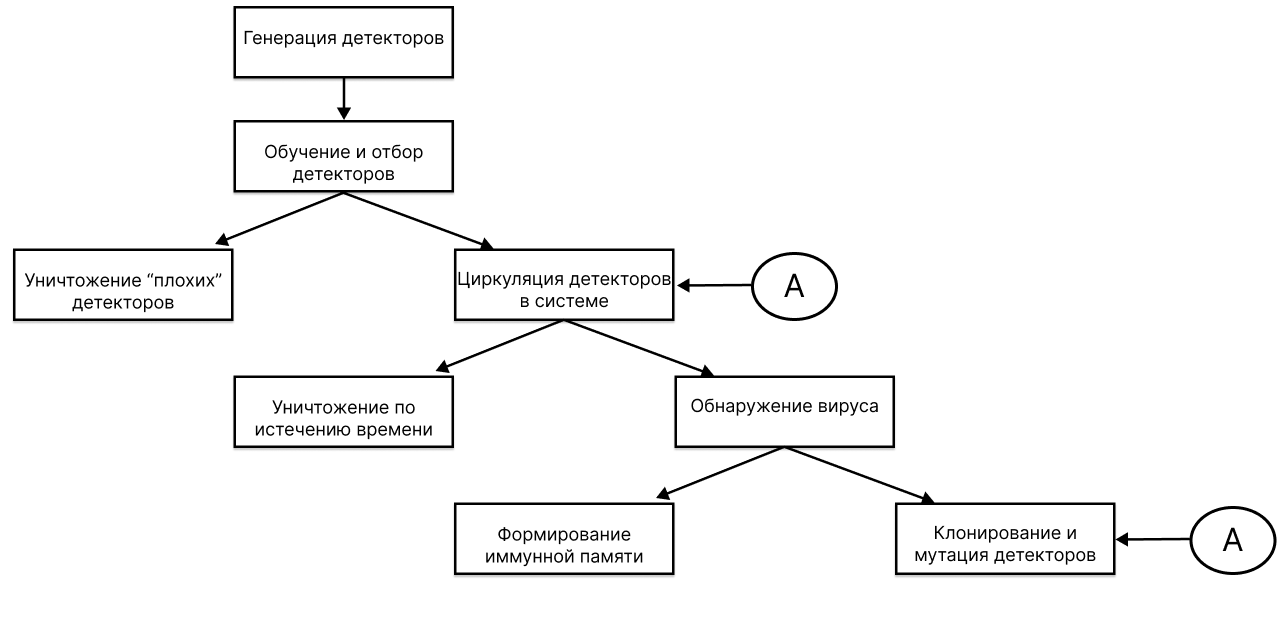
\includegraphics[width=0.7\textwidth]{pics/1.png}
    \caption{Взаимодействие процессов искусственной иммунной системы}
    \label{s1}
\end{figure} 

\subsection{Роль ИИС в обнаружении и борьбе с угрозами}

\section{Нейронные иммунные сети}

\subsection{Внедрение }
\subsection{}


\subsection{Перспективы нейронных иммунных сетей}


\begin{thebibliography}{15}
    \bibitem{ais1}
    Remote Utilities RDP [Электронный ресурс] : подключение к удаленному рабочему столу. --  
    Remote Utilities Pty (Cy) Ltd 2010 -- 2023. -- URL:  https://rep.bstu.by/bitstream/handle/data/37388/79-88.pdf?sequence=1 (дата обращения: 31.12.2023). -- Загл. с экрана. -- Яз. англ.
    
    \bibitem{ais2}
    https://rep.bstu.by/bitstream/handle/data/1179/3-5.pdf?sequence=1
\end{thebibliography}


\end{document}